\documentclass[UTF8]{article}
\usepackage[utf8]{inputenc}
\usepackage[no-math]{fontspec}
\usepackage{fdsymbol}       
\usepackage{newunicodechar} 
%\usepackage[T1,T2A]{fontenc}
%\usepackage[english]{babel}
%\usepackage{CJKutf8}
\usepackage{ctex}
%\usepackage[no-math]{fontspec}
%\usepackage{xeCJK}

%\usepackage{amsmath}
%\usepackage{amssymb}
%\usepackage{tikz}
\usepackage{enumitem}
\usepackage{graphicx}
\usepackage{multicol}

\usepackage{wrapfig}
\graphicspath{ {./pic/} }

\usepackage{hyperref}
% \hypersetup{
%     colorlinks=true,
%     linkcolor=black,
%     filecolor=magenta,      
%     urlcolor=cyan,
% }

% black text on white background
\usepackage{xcolor}
\usepackage{pagecolor}
\usepackage{mdframed}
\pagecolor{white}
\color{black}

% better font
\usepackage[defaultsans]{droidsans}
\renewcommand{\sfdefault}{ptm}


\usepackage[a4paper]{geometry}
\usepackage{filecontents, pgffor}

\usepackage[backend=biber]{biblatex}
\addbibresource{Mendeley.bib}
\usepackage{csquotes}
%\setCJKmainfont{simsun.ttf}

% Copyright 2017 Sergei Tikhomirov, MIT License
% https://github.com/s-tikhomirov/solidity-latex-highlighting/

\usepackage{listings, xcolor}

\definecolor{verylightgray}{rgb}{.97,.97,.97}

\lstdefinelanguage{Solidity}{
	keywords=[1]{anonymous, assembly, assert, balance, break, call, callcode, case, catch, class, constant, continue, contract, debugger, default, delegatecall, delete, do, else, event, export, external, false, finally, for, function, gas, if, implements, import, in, indexed, instanceof, interface, internal, is, length, library, log0, log1, log2, log3, log4, memory, modifier, new, payable, pragma, private, protected, public, pure, push, require, return, returns, revert, selfdestruct, send, storage, struct, suicide, super, switch, then, this, throw, transfer, true, try, typeof, using, value, view, while, with, addmod, ecrecover, keccak256, mulmod, ripemd160, sha256, sha3}, % generic keywords including crypto operations
	keywordstyle=[1]\color{blue}\bfseries,
	keywords=[2]{address, bool, byte, bytes, bytes1, bytes2, bytes3, bytes4, bytes5, bytes6, bytes7, bytes8, bytes9, bytes10, bytes11, bytes12, bytes13, bytes14, bytes15, bytes16, bytes17, bytes18, bytes19, bytes20, bytes21, bytes22, bytes23, bytes24, bytes25, bytes26, bytes27, bytes28, bytes29, bytes30, bytes31, bytes32, enum, int, int8, int16, int24, int32, int40, int48, int56, int64, int72, int80, int88, int96, int104, int112, int120, int128, int136, int144, int152, int160, int168, int176, int184, int192, int200, int208, int216, int224, int232, int240, int248, int256, mapping, string, uint, uint8, uint16, uint24, uint32, uint40, uint48, uint56, uint64, uint72, uint80, uint88, uint96, uint104, uint112, uint120, uint128, uint136, uint144, uint152, uint160, uint168, uint176, uint184, uint192, uint200, uint208, uint216, uint224, uint232, uint240, uint248, uint256, var, void, ether, finney, szabo, wei, days, hours, minutes, seconds, weeks, years},	% types; money and time units
	keywordstyle=[2]\color{teal}\bfseries,
	keywords=[3]{block, blockhash, coinbase, difficulty, gaslimit, number, timestamp, msg, data, gas, sender, sig, value, now, tx, gasprice, origin},	% environment variables
	keywordstyle=[3]\color{violet}\bfseries,
	identifierstyle=\color{black},
	sensitive=false,
	comment=[l]{//},
	morecomment=[s]{/*}{*/},
	commentstyle=\color{gray}\ttfamily,
	stringstyle=\color{red}\ttfamily,
	morestring=[b]',
	morestring=[b]"
}

\lstset{
	language=Solidity,
	backgroundcolor=\color{verylightgray},
	extendedchars=true,
	basicstyle=\footnotesize\ttfamily,
	showstringspaces=false,
	showspaces=false,
	numbers=left,
	numberstyle=\footnotesize,
	numbersep=9pt,
	tabsize=2,
	breaklines=true,
	showtabs=false,
	captionpos=b
}

% Python style for highlighting
\newcommand\pythonstyle{\lstset{
    language=Python,
    basicstyle=\ttm,
    otherkeywords={self},             % Add keywords here
    keywordstyle=\ttb\color{deepblue},
    emph={MyClass,__init__},          % Custom highlighting
    emphstyle=\ttb\color{deepred},    % Custom highlighting style
    stringstyle=\color{deepgreen},
    frame=tb,                         % Any extra options here
    showstringspaces=false            % 
}}


% Python environment
\lstnewenvironment{python}[1][]
{
    \pythonstyle
    \lstset{#1}
}
{}
	% copy the file from this repo

%\selectlanguage{english}

\title{Robonomics:将网络物理系统整合到人类经济中的平台 \\ \small
\textit{适用于工程师,智能城市和工业4.0创作者}}
\date{2018年5月12日}

\author{Sergey Lonshakov \\ Aleksandr Krupenkin \\ Aleksandr Kapitonov, PhD \\ 电子邮箱: \href{mailto:research@aira.life}{research@aira.life} \and Evgeny Radchenko \\ Alisher Khassanov \\ Aleksandr Starostin \\ 电子邮箱: \href{mailto:engineering@aira.life}{engineering@aira.life} \and Translated by Nikolay Kapustin 电子邮箱: \href{mailto:nikolaykapustin4@gmail.com}{nikolaykapustin4@gmail.com} }

\begin{document}
%\begin{CJK}{UTF8}{bsmi}
\maketitle
 
\begin{abstract}
在生产,物流和城市生活中全面使用网络物理系统(CPS)将使我们能够应对日益复杂的供应链,并为消费者提供优质产品。 根据文章作者的说法,这里的主要问题是安排不同CPS的全球合作。

我们认为安排自主网络物理系统的协作作为基于市场机制的网络是最可持续的选择。

可以在p2p技术的基础上创建基于市场机制建立并且最终用户可直接访问的适应人类需求的网络物理系统的分发,控制和提供服务的网络。 这允许将交易的技术和经济参数在机器上组合。

构建这样的对等网络可以在以太坊基础设施的基础上进行。 通过扩展基本通信协议的功能,我们可以训练网络物理系统与市场机制和合同义务相互作用。

创建和开发一个平台,提供与机器人经济网络合作的工具(简称 -  Robonomics平台)将允许新城市和工业区的设计师在自动机器人服务之间建立信任,为从自治工厂和城市传感器网络服务订购产品提供直接用户访问。这反过来将使我们能够建立一个全球监控网络物理系统活动的分散系统。
\end{abstract}

\tableofcontents

\section{介绍}
由于机器人系统的巨大潜力,预计在不久的将来\cite{Pedersen2016RobotDeployment}将对大多数生产过程进行全球变更。 机器人系统能够适应\cite{Stock2016Opportunities4.0}广泛的任务,在许多类型的经营活动中更有效,并且减少了生产的时间支出。 生产的机器人化正在增长:从2015年到2016年,每10,000名企业员工的世界平均机器人单位数增加了11% \cite{2018RobotRobotics.}。 例如,仅在2017年的中欧和东欧,他们装备的机器人单位比2016年增加了28% \cite{2018EnterFactories} 。大多数企业家在机器人技术中看到了提高生产效率和弥补人员短缺的可能性 \cite{2018EnterFactories} 。

有必要明确如何预测大规模引入机器人系统。 计算设备系统一方面通过网络服务相互协作以进行访问和数据处理,另一方面主动与周围物理世界交互,似乎是网络物理系统(CPS)的概念\cite{Kang2016SmartDirections}。 除了自动机器人之外,这一概念的主要技术趋势是大数据,物联网,云计算等。网络物理系统是工业4.0 \cite{Jazdi2014Cyber4.0}的概念关键要素 - 第四次工业革命,即 由于CPS的引入。 预计这些变化的规模如此之大,以至于它们不仅影响和改变生产方法\cite{MonostoriLaszlo2014Cyber-physicalChallenges} ,而且影响和改变人类从事工业的基本原则。

因此,这些全球变化给科学家和开发人员带来了许多新的挑战。 自动化代理引入(我们将机器人系统,智能事物和软件代理结合到这个概念中)的重要问题之一 \cite{Leitao2015IndustrialIndustry} 是生产,并且机器人领域的研究人员正在考虑 \cite{Zhu2014RobustSystems} 这个问题是组织联合和功能性工作的问题 一个多代理者 \cite{Liu2013Multi-robotConstraints} 。 此外,现代工业的具体特征 \cite{Lasi2014Industry4.0} 导致组织的集中结构面临与失败 \cite{Khajavi2014AdditiveChain},错误或黑客风险相关的巨大成本。 研究人员认为,分布式生产方法变得更加实用:由此,交易成本(承包成本),运输成本,存储成本和设备过时成本降低。 因此,分散式系统在生产中是最有前途的 \cite{DeGennaro2006DecentralizedSystems}。

比特币创造了一个网络,机器人可以参与人类社会的经济环境。 机器有机会在没有人工直接帮助的情况下交换价值。 换句话说,比特币成为机器人的第一笔钱\cite{Kelion2015CouldThemselves}。

以太坊网络的推出使我们能够通过智能合约扩大机器人经济上有意义的沟通的可能性\cite{Buterin2014EthereumPlatform}。 智能合约现在允许我们将金融交易的技术细节添加到机器。


从消费者到网络物理系统运营商的经济上有意义的交易,以及从服务员到服务器应该提供的机器人的技术交易,我们现在可以利用以太网网络智能合约提供的机会,而不是两笔交易。 从消费者直接到网络物理系统的交易。

\textit{机器人现在能够执行合同条款中指定的程序,并根据其工作创建标记化值。}

由于Wiener \cite{Wiener1961CyberneticsEd} 和 Glushkov \cite{SergienkoIvan2014TopicalGlushkov} 对控制论发展的贡献以及Coase \cite{Coase1937TheFirm} 对理解公司性质的贡献,我们可以讨论通过市场机制建立网络来管理智能城市和工业4.0中的网络物理系统的可能性。

\section{机器人的经济}

经济理论从无限的需求和有限的资源的角度来处理剥削问题。 社会对自动化的渴望是解决资源合理或更有效支出问题的一个要素,以满足日益增长的需求。 我们实际上无法通过今天消费的手工劳动来生产尽可能多的商品和服务。 除量化指标外,质量问题也非常重要; 货物本身的复杂性和确保对其生产的控制超出了人的能力范围。 微电子生产,重工业和制药业是没有机器参与的当今世界无法生存的行业。

全自动化企业的出现在当今工业区的现代城市运营和生活中是不可避免的。 这些企业由网络物理系统控制,并代表其作为自主代理的服务。 从自主CPS形成网络的过程也是不可避免的,并且对于提高服务的生产和呈现过程中的通信速度和质量至关重要。 我们保护市场机制是建立网络物理系统网络的力量。 一方面,市场将使CPS网络适应个人不断变化的需求。
另一方面,它将作为自主代理人的经济效率来规范CPS的规模。

在市场机制的帮助下整合CPS使我们有机会实施直接融入社会经济的全球商品和服务大规模生产系统。 该系统即机器人网络的经济性。

\section{网络物理系统的想法}

重要的是要考虑到,在设计机器人服务时,使用市场机制进行网络集成强制要求将CPS表示为经济代理。 与罗纳德科斯在他的文章“公司的本质”中所描述的公司在市场上出现的过程类似,可以考虑将网络物理系统演变为自治经济主体。 市场机制的成本和机会正在CPS中引入经济博弈。 这创建了一个过滤器,消除了经济上低效的机器人服务的通信可能性。 这也消除了CPS扩大到导致其存在的风险和不必要的成本超过社会集中系统的可能性。

\textit{与经济中的公司类似,网络物理系统(CPS)将许多机器人集成到能够进行有组织协作的紧密连接的传感器和执行器网络中。}

\section{机器的责任}

\textit{我们生活在权利和责任的世界里。 如果人类在机器人默认获得某些权利时没有看到优势,那么人们肯定会对机器上的负债感兴趣。}

捍卫市场机制作为自治CPS网络中的通信手段,我们必须确定与机器达成协议的主题。

在生产商品和提供服务的过程中,机器实际上无法以与人类相同的方式感知协议的主题。 如果我们考虑17世纪后经济理论的第一次变化并回顾马歇尔的价格理论,我们会注意到消费者对商品价值的看法是基于对实际个体经济中商品利益的主观感知。 同样,生产者对同一商品价格的评估源于生产成本。 在这方面,我们可以说,在今天的人类社会中,对消费者和生产者来说,商品或服务的看法是不同的。

机器不会闲聊。 如果您与机器签订了合同,那么它将执行其程序。 在处理CPS时,可能会排除与人们执行某项任务的动机相关的风险。 在这种情况下,我们可以使用义务来执行CPS行为的某种模型,其中用户数据作为与机器的交易的主体。 通过评估已经实施的不同CPS行为模型的消费者质量结果,我们将观察同一商品或服务市场中各种机器行为模型的投标价格范围。 这些信息足以投资于机器人技术的开发,以实现越来越完美无瑕和复杂的CPS行为模型。

通过让机器承担责任并为其服务创造责任,我们可以将经济自主的代理完全整合到消费者环境中。 这种责任的主体应该是行为模型的实施,这将实现消费者的需求。 例如,想象一下自动售货机从办公室工作人员那里收取费用,转而支持在数字市场上为城市的服务和商品提供自助服务。

考虑到其通信的技术和经济参数的CPS行为模型或程序可以作为机器人经济市场中的标准化产品呈现并表示为合同责任。

\section{Robonomics 平台}

我们正在考虑一种允许我们使用现有技术组织机器人经济学网络的方案。 根据2015年至2018年间进行的实验结果,我们提出以下建议:使用以太坊作为基础设施,提供最低限度的必要设施,将机器的技术和经济参数结合起来,实现行为模型。 与用户协调。 作为Robonomics平台考虑的一部分,我们是:

\begin{itemize}[noitemsep]
	\item 扩大以太坊的能力,以便CPS市场的行为模型供需出现;
	\item 将Robonomics代理操作系统描述为机器人操作系统兼容的CPS与机器人经济网络的接口\cite{Quigley2009ROS:System};
	\item 举例说明Robonomics平台应用程序,用于实现Smart Cities和Industry 4.0的用户dapp SDK开发人员。
\end{itemize}

\subsection{以太坊区块链交易和责任合同}

当供应满足Robonomics的需求时,交易将被发送到以太坊区块链,并且它们完全满足彼此的条件。 在这种情况下,Robonomics为以太坊平台参与者创建了一条消息。 此消息包含合同工厂创建机器人责任合同所需的参数。

\subsubsection{合同工厂}

在以太坊网络中创建智能合约有两种方法:
\begin{itemize}[noitemsep]
	\item 使用特殊事务下载合同代码:
	\item 从另一个合同创建合同
\end{itemize}

在第一种情况下,外部帐户从源文本编译合同并将其代码发送到事务。 这要求用户拥有编译器和一组源文本,这会给最终用户和自动化系统带来困难。

让我们考虑一个更有趣的第二个选择:当以太坊网络中的合同自己创建合同时,测试给定的条件。 我们将此机制称为合同工厂。

\begin{lstlisting}
contract A {}

contract B {
  function foo() {
    var a = new A();
    ...
  }
}
\end{lstlisting}

在上面的示例中,合同代码A完全包含在合同代码B中。

\subsubsection{轻量级合同}

有时工厂可以创造太多的智能合约。 在这种情况下,在部署新合同时,不仅会分配用户数据的空间,还会复制代码。 这燃烧气体并堵塞区块链。

让我们考虑一种非常强大的技术。 在EVM指令集中,有一个DELEGATECALL操作码,允许在当前合同的上下文中执行外部代码。 这种方法称为共享代码合同。 见下图。

让我们假设有用的契约只包含用户数据,与共享代码的契约包含处理它的方法。 使用DELEGATECALL操作码,我们可以采用从一个通用契约处理用户数据的方法,极大地促进了多次复制的有用契约。 为此,只需在有用的合同中添加回退方法即可。

\begin{lstlisting}
function () {
 require(shared.delegatecall(msg.data));
}
\end{lstlisting}

这是与共享代码签订合同的地址。 有用合同无法处理的所有交易将被代理到保存上下文的一般合同。 使用共享代码复制合同的技术更有用,并且在更频繁的基础上计划创建新合同。 例如,对于机器人责任合同,此方法允许每次交易节省30-40%的气。

\subsubsection{基于延迟签名创建合同}

以太坊支持椭圆曲线上的数字签名,即ecrecover功能。 这样的功能允许我们从随机数据的签名中恢复公钥,即以太坊地址。

\begin{lstlisting}
contract Checker is owned {
    function byOwner(bytes32 _message, uint8 _v, bytes32 _r, bytes32 _s) view returns (bool) {
        return ecrecover(_message, _v, _r, _s) == owner;
    }
}
\end{lstlisting}

在上面的示例中,当且仅当消息使用合同所有者的私钥签名时,byOwner方法才会生效。 要签署消息,以太坊网络的热门客户端提供eth.sign(帐户,消息)方法。 例如,数字签名可用于创建合约,合约的各方不是交易的发件人,但指定其参数。

\begin{lstlisting}
var promisee = ecrecover(keccak256(MSGPREFIX, askHash), uint8(_sign[1]), _sign[2], _sign[3]);
var promisor = ecrecover(keccak256(MSGPREFIX, bidHash), uint8(_sign[5]), _sign[6], _sign[7]);
var inst = new RobotLiability(_model, _objective, promisee, promisor, _param[0], _param[1], _param[2]);
\end{lstlisting}

负债工厂从数字签名恢复交易发件人的地址。 可靠地想要签订此合同的地址可以在机器人责任合同中获得。 交易发件人与其他方之间可能不存在信任。 在这种情况下,交易的发送者不能通过替换交易参与者的地址来执行任何欺诈,因为该地址没有明确地出现在交易参数中。

数字签名机制与智能合约一起允许我们将交易发送者的角色委托给第三个不受信任的一方。

\subsection{供应商和灯塔}

在以太坊区块链中Robonomics网络的经济上有意义的数据的位置需要分配将承担此功能的特殊参与者组; 即机器人网络经济的提供者。

灯塔是一种自主工作流程,允许我们分配服务于单个广播频道的提供商的运行时间。 让我们区分两组Robonomics网络节点:

\begin{enumerate}
   \item 普通网络参与者 - 对Robonomics网络服务感兴趣的节点:
   \begin{itemize}
     \item 发送需求和/或供应信息以执行CPS计划;
     \item 在程序执行时发送CPS的结果(协议);
     \item 接收来自其他参与者的消息;
     \item 将消息转发给其他参与者。
   \end{itemize}
   \item 提供商 - 对以太坊区块链中Robonomics网络经济上有意义的信息位置感兴趣的节点:
   \begin{itemize}
     \item 接收来自其他参与者的消息;
     \item 将消息转发给其他参与者;
     \item 一旦在渠道中找到匹配的供需,就找到有关交易的信息;
     \item 一旦从观测网络中找到确认信息,就会将信息放在工作结果上。
   \end{itemize}
\end{enumerate}

让我们区分灯塔支持的两类责任合同交易:

\begin{enumerate}
	\item 根据Robonomics市场的供需比较开立(创建)合同;
	\item 根据观察网络确认的工作结果,完成合同的终止(最终确定)。
\end{enumerate}

灯塔提供商的经济游戏包括以下内容:

\begin{enumerate}
	\item 寻找匹配的供需,目的是创建合同责任的交易地点。 灯塔将获得用户提议的总佣金;
	\item 寻找确认的工作结果,目的是确定责任合同的交易地点。 灯塔将获得赔偿责任最终确定的令牌排放奖励。
\end{enumerate}

\subsection{Robonomics 计划}

Robonomics程序是位于以太坊区块链上的工作流程,供应商可以通过该工作流程根据交易的技术和经济参数执行CPS行为模型。

Robonomics程序的执行可以有条件地分为两个阶段:

\begin{enumerate}
	\item 责任的起始
	\item 责任的最终确定
\end{enumerate}

在Robonomics程序实施的阶段(1)期间,基于两个延迟签名恢复初始化合同责任所需的数据。 每个延期签名必须包含:
\newline
\newline

\begin{tabular}{ |l |l |l }
 \textbf{Field} & \textbf{Type} & \textbf{Description} \\ 
 \hline
 model & bytes32 & CPS行为模型的标识符(哈希值) \\  
 objective & bytes32 & CPS行为模型的参数(哈希值)(可选) \\
 token & address & 操作代币(以太坊地址) \\
 cost & uint256 & CPS行为模型实施的成本(数量) \\
 count & uint256 & CPS行为模型执行次数(数量) \\
 lighthouseFee & uint256 & 灯塔网络佣金(编号) \\
 validator & address & 观察网络地址(以太坊地址) \\
 validatorFee & uint256 & 观察网络佣金(数量) \\
 salt & bytes32 & Salt(随机数据) \\
 signature & bytes & 发件人数字签名(数据) \\
\end{tabular}

通过模型,代币,价格和执行次数协调的2个递延签名,我们可以发送Robonomics合同工厂的智能合约交易,该合约将:

\begin{enumerate}
	\item 从签名中检索数据;
	\item 创建新的智能合约责任;
	\item 在指定的代币中转移所需的安全性;
\end{enumerate}

在阶段(2)期间,提供商通过向包含操作日志的哈希的CPS发送延迟签名来最终确定责任合同,这导致:
\begin{enumerate}
	\item 哈希记录在字段中,负责存储责任执行的结果;
	\item 将位于责任合同中的代币转移到参与者的地址。
\end{enumerate}

\subsection{Robonomics代理操作系统}

Robonomics操作系统的基本和最重要的功能是启动网络物理系统程序,其参数由用户在智能合约中设置。

Robonomics OS的目的是为网络物理系统提供软件,这是进行经济上有意义的交易以及使用p2p网络发送和接收消息所必需的。

\subsubsection{应用配置和OS生成}
当程序很简单,640千字节对每个人都足够时,通常通过复制到用户的PC来完成软件分发。 复制的实践需要许多明显的问题:更新,依赖,文件系统混乱等。为解决这些问题,已经发明了特殊程序:包管理器。 他们负责跟踪更新,依赖关系,会计变更等等。 这种具有命令式方法的包管理器现在无处不在,但还有另一种方法。
让每个包在目标系统上保持隔离,永远不会被过度记录。 通过哈希和确认文件的完整性。 通过类比功能语言的含义,让包由纯函数收集; 没有副作用的功能。 这将给我们带来许多有趣的后果:
组件的可重复性。 纯函数将始终在给定的参数上返回相同的结果,因此包将始终以相同的方式形成;

\begin{enumerate}
\item 组件的可重复性。 纯函数将始终在给定的参数上返回相同的结果,因此包将始终以相同的方式形成;
\item 缓存。 没有必要每次都收集包,清洁度允许我们将包保存在二进制缓存中(并允许访问其他参与者);
\item 依赖。 更改包参数中的依赖关系(例如,更新版本)会导致输出和重建的更改。 如果这个包也是某人的依赖,这反过来导致递归重建。
\end{enumerate}

在大多数现代操作系统上,部分更新会使系统处于不一致状态,并且可能不再启动。 这种情况在机器人分布式控制系统和实时服务中是不可接受的。 由于采用纯函数方法,新配置(称为build)不会过度记录旧配置,因此始终可以原子地回滚更改并返回到工作状态(build)。

返回到原始状态非常快,并且由于不需要从上一代下载包,因此它们已经存储在系统中不变。 有大量的机器人系统,以及描述和建模它们的方法。 从实际的角度来看,这导致出现了一整套彼此不兼容的库,程序和框架,并且不适用于不同类的机器人系统。 在这种情况下,唯一适当的解决方案是为机器人技术中的控制系统开发开放式通信标准。

这样的标准被提议作为开放项目机器人操作系统的一部分。 这些表示由两种格式组成的通信:面向事件的PubSub和客户端 - 服务器服务。 数据格式在一系列软件和库中形式化,形成围绕管理系统通信的集成方式的开放社区和基础设施。

支持机器人内部控制系统通信的集成标准是Robonomics分发包的重要任务。 作为此任务的一部分,将执行几个步骤:准备,移植和在Robonomics OS的参考实现中包含ROS元素 - AIRA。

\subsubsection{执行智能合约中描述的程序}

机器人责任合同是为了形式化执行而创建的,并且由网络物理系统的用户行为参数化。

合同字段模型中描述了一般行为模型。
\begin{lstlisting}
bytes public model;
\end{lstlisting}

这是位于分散数据存储中的IPFS哈希文件。 与网络的任何其他参与者一样,机器人可以在本地下载此文件并解释其内容。 模型文件内容的示例:

\begin{lstlisting}
 {
    parity.enable = true;
    parity.chain = "kovan";

    railway-game.enable = true;
  }
\end{lstlisting}

这些是函数式语言Nix \cite{Dolstra2010NixOS:Distribution}中的指令,它们包含在Robonomics OS配置中,用于激活给定行为模型的软件。 这里,例如,激活KOVAN网络中的以太坊节点服务和“火车游戏”测试台的服务。

行为模型描述了软件结构和静态参数,其存在是系统执行所需动作所必需的。

用户参数在责任合同中单独转移,也在现场目标中转移。 这是位于分散存储库中的文件的IPFS哈希值。 文件格式符合ROSBAG v2规范(http://wiki.ros.org/Bags/Format/2.0),并定义了网络物理系统行为的动态参数。 BAG文件在机器人履行责任时播放,并使用数据参数将消息传递给正在运行的系统。 这些参数既可以扮演执行触发器的角色,又可以优化所需服务或产品的特性。 例如,工厂工厂“正在使用的工业4.0”的消息包含以下消息:

\begin{tabular}{ |l |l |l }
 \textbf{Topic} & \textbf{Type} & \textbf{Value} \\ 
 \hline
 model & bytes32 & CPS行为模型的标识符(哈希值) \\ 
 - &  - & data: “blue” \\ 
\end{tabular}

与接收消息相关联的事件用作智能工厂履行责任以生产产品的触发器,并且消息的内容指定其特征。

在用户参数再现开始时,网络物理系统操作协议也开始。 然后,以ROSBAGv2格式的操作日志的形式将网络物理系统操作的结果加载到分散的存储库中。 文件的IPFShash(地址)被发送到智能合约,作为对网络物理系统执行的工作的确认。 监控机器人负债履行情况的任务由独立的节点网络处理,这些节点根据责任合同解释工作协议。

\subsection{观察网络}

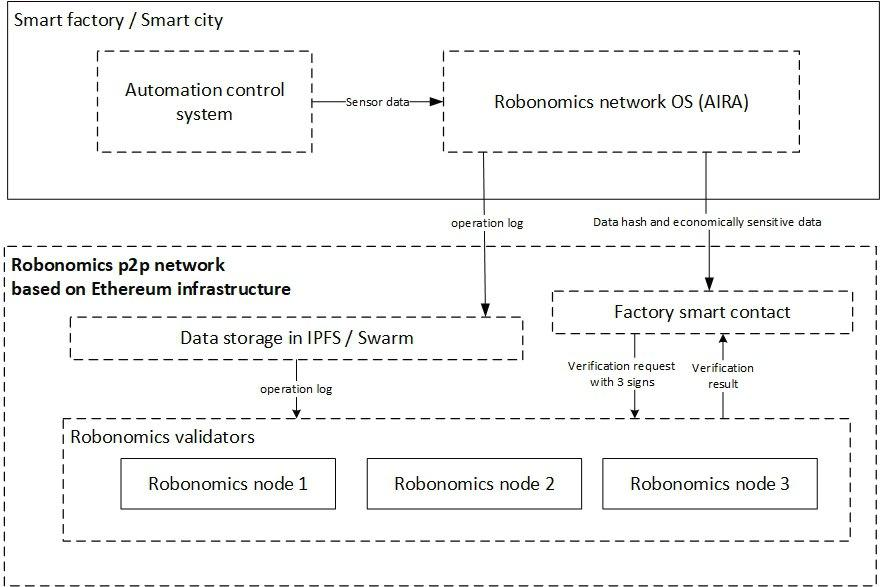
\includegraphics[width=1\textwidth]{app-3.png} 

Robonomics能够通过验证机器工作结果的验证模型来监控机器人合同责任的性能。 为此,合同责任必须表明所需的观测网络和验证模型。

根据工程师和机器人使用的框架的行为模型是工作绩效的主要元素。

\subsubsection{观察者契约的工作算法}

合同初始化的方式与灯塔合同的初始化方式相同; 参与者按照发放负债核实配额的比例向合同存入担保。
\begin{enumerate}
	\item 在结果渠道中,会显示一条消息,其中包含要求验证人确认的责任结果。
	\item 观察网络的参与者使用标记来对消息进行结果签名,并通过其决定将其发送到结果通道。
	\item 灯塔捕获带有验证器确认的消息,但它不能位于N个块中。
	\item 如果观察网络中的其他参与者不同于标记的当前所有者,则他们可以将他们的决定发布到结果通道。
	\item 如果根据未与标记的当前所有者讨论的决定达到BFT,则该交易可立即置于责任合同中,并且标记的当前所有者将失去配额。
	\item XRT的手续费被转移到观察网络的参与者,以核实合同责任。
\end{enumerate}

\section{Robonomics 代币, XRT}

Robonomics代币的任务是确保分散网络的运行,以维护以太坊基础设施中的智能城市和工业4.0。 为了实现这一目标,代币经济需要反映独立提供商实施网络有用功能的动机。 这些激励措施应在排放和佣金之间分配,以确保以太坊中Robonomics的能力取决于XRT代币的价格,以及激励供应商使用用户提供的数据在EVM中运行Robonomics计划。

\subsection{在以太坊计算机中执行Robonomics程序的排放}

比特币和以太坊的排放有一个有趣的特征:无论是否有交易,仍然会创建块。 这种相对“无差异”允许网络根据通信协议保证其容量。 排放是矿工维持特定吞吐量的关键动力,而无需等待区块中有利可图的总佣金的积累。
 
将Robonomics表示为EVM程序允许我们将XRT标记的排放与循环气体的量连接起来作为评估计算和保存以太坊计算机中任何程序的数据的常用指标。 这将确保整个以太坊基础设施中的Robonomics容量与XRT代币的价格相关。

让我们介绍Robonomics的基本技术单元Wiener(1 XRT = $10^9$ Wn)并定义它的以下功能: 
\\
\\
\textit{Robonomics使用的1 Wn = 1气体的排放}
\\
\\
这种模式规定:
\begin{enumerate}
	\item XRT不等于1 ETH,因为1气体可能花费不同的wei量。
	\item 1 Wn的成本必须包括在以太坊处置1单位天然气的供应商的成本。
	\item 只有Robonomics程序应该能够执行Wn发射。
	\item XRT价格的任何增加都将有助于增加Robonomics的产能。
	\item XRT的总资本化可能大于ETH的资本化,因为它除了在EVM中使用天然气之外还具有额外的功能。
\end{enumerate}

为了实现Robonomics使用的1 Wn = 1气体的排放率,我们提供:

\begin{enumerate}
	\item 在TGE期间,通过荷兰式拍卖,找到最初的Wn排放乘数,以涵盖供应商的最低必要费用,以确保在发射的最初时刻在以太坊基础设施中存在Robonomics。
	\item 介绍网络开发阶段,在此期间,排放乘数将根据EVM中Robonomics程序执行中使用的气体总量进行算法减少。
	\item 将来,确保以色列Robonomics公司为每个使用过的气体单位提供永久的Wn排放。
\end{enumerate}

\subsubsection{TGE和荷兰式拍卖}

在Robonomics推出的最初时刻,我们建议发行10,000,000 XRT,其中5%至77%将用于荷兰式拍卖。我们为募捐活动设定了N ETH的目标,该活动将针对特别创建的Robonomics基金会的账户,该基金会将支持开发代表CPS作为经济自主代理商的基本概念。世界上可供使用的经济自主代理商的模型越多,使Robonomics一般工作的可能性就越高。作为拍卖的结果,所有参与者将以尽可能低的价格获得代币,而Robonomics将获得XRT与ETH的初始比率。将这些数据与当前的天然气价格统计数据相结合,我们将能够确定以太坊基础设施中Robonomics开发期间的初始排放乘数,以便以有竞争力的价格支付供应商的成本,因为资本化自然较低Robonomics与初始阶段的以太坊相比。根据我们对2018年春季的计算,以太坊网络的最低​​竞争价格是每1气体2 gwei的价格。

\subsubsection{发展}

我们将以太坊基础设施中Robonomics开发的时期划分为5个时期,每个时期在以太坊的使用天然气总量中进行统计估算。 在结束时,时期在算法上以这样的方式减少排放乘数:在开发期结束时,满足以下条件:
\\
\\
\textit{Robonomics使用1 wn = 1气体的排放}
\\
\\
也就是说,乘数应该减少到1,在过去消失。
\\
\\
下面是Robonomics开发的五个时期的参数表:
\\
\\
\begin{tabular}{ |l |l |l |l}
 \textbf{时代} & \textbf{利用天然气} & \textbf{E(i), Wn} & \textbf{E(i), XRT} \\ 
 \hline
 1 &  3,47E+12 & 2,08E+13 & 2,08E+06 \\ 
 2 &  3,47E+12 & 1,39E+13 & 1,39E+06 \\ 
 3 &  3,47E+12 & 9,26E+12 & 9,26E+05 \\ 
 4 &  3,47E+12 & 6,17E+12 & 6,17E+05 \\ 
 5 &  3,47E+12 & 4,12E+12 & 4,12E+05 \\ 
 总共 &  1,74E+13 & 5,43E+13 & 5,43E+06 \\ 
\end{tabular}

我们允许块中的气体量作为恒定值,因为实际上不可能预测其今天的增长。 因此,我们只能判断每个时期的过境意味着根据以太坊中2018年春季时段的大小数据利用天然气的百分比。在第五个时代结束时,我们可以说 Robonomics已经达到了2018年春季在以太坊网络上可用的一年度天然气量的指标。无论如何,这些统计数据足以根据2018年TGE时刻对Robonomics增长进行客观评估。

\subsubsection{进一步排放}

在经过开发阶段后,Robonomics将达到恒定的排放量,其定量等于Robonomics使用的1 Wn = 1气体的所需指标排放。 这种线性关系将有助于确保提供商在没有佣金的情况下均衡Robonomics的资本化后可以确保的最低容量。

\subsection{在以太坊基础设施中启动Robonomics计划的费用}

Robonomics计划的实施与模拟EVM的实际参与者之间的第一个区别是从创建CPS的合同义务到发送工作产品和完成程序执行的那一刻无限期的时间, 这是基于此交易。 这意味着CPS应该有兴趣向网络支付佣金,包括提供商在通信渠道中工作的费用,以找到具有协调供需的CPS,以及解决交易以产生合同义务的成本 在以太坊区块链中。

\subsection{XRT代币其他任务}
\subsubsection{用户委托使观察网络存在}

考虑到观测网络,没有必要激励提供商最终完成Robonomics计划的实施。 任何提供商都会为了排放而愉快地完成Robonomics计划的实施。 因此,CPS服务用户佣金只能用于支付CPS行为模型执行结果的验证。

\subsubsection{XRT作为Robonomics的信任机制在灯塔上积累}

在Robonomics存在的零时间,供应商将有兴趣以安全的形式创建灯塔合同的最低XRT率的“个人”灯塔。 一旦Robonomics出现供需,对特定灯塔的兴趣将会更高,并且提供商可以从这个特定灯塔所服务的通信渠道获得的总佣金将更大。 随着时间的推移,供应商将开始围绕这些灯塔进行整合,其中提供商在灯塔合同上的安全份额将给予足够的时间来获得额外的好处。 最终,某些通信渠道的总佣金越高,提供商准备冻结的XRT份额就越大。 特定灯塔的冻结资金数量越大,其他参与者对灯塔运营和Robonomics的信任程度就越高。

\subsubsection{XRT作为网络资本的定量反映}

Robonomics资本只不过是使用以太坊基础设施建立与经济自主CPS通信的网络价值的反映。
 
这样一个网络的资本增长将代表社会中接受CPS作为自治经济主体的人数的增长。 另一方面,以太坊将被视为适用于基于学术和工业自动化标准的经济上有意义的通信的基础设施。

\subsubsection{控制市场}

从长远来看,XRT将成为合同机器人到机器人负债市场的内部货币,最初是CPS签订合同义务并验证其结果所必需的代币。 这将是每个程序执行将循环到程序执行的市场。

\subsubsection{关于XRT在Robonomics网络中运动的结论}

总而言之,这就是我们所拥有的:XRT排放旨在保持Robonomics不断准备好与CPS作为以太坊基础设施中的自治经济代理执行通信。 手续费激励供应商在执行Robonomics计划时使用用户数据。

\subsubsection{面值}
\begin{tabular}{ l |l |l |l |l}
 价值 &  $1$ & $10^3$ & $10^6$  & $10^9$ \\ 
 \hline
 Robonomics平台的标题 &  wiener & coase  & glushkov & robonomics token\\ 
\end{tabular}

\section{Robonomics工作的描述}
\subsection{工程师提出的新行为模型的建议}

\begin{wrapfigure}{l}{0.30\textwidth} %this figure will be at the right
    \centering
    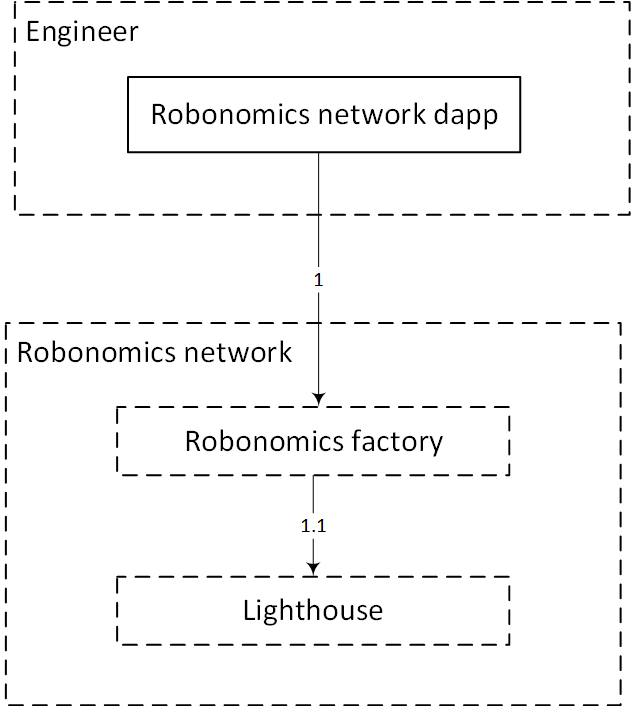
\includegraphics[width=0.30\textwidth]{step-by-step-1.png}
\end{wrapfigure}

自治工作流程中的灯塔,允许分发提供商工作时间并为特定广播频道提供服务。

Robonomics工厂是一个自主的工作流程,允许使用存储在以太坊区块链上的相应库创建新的灯塔或责任合同。

创建网络物理系统的组织可能有兴趣将其机器人作为可以管理其自身经济的服务来呈现:从提供服务之前获取技术和财务参数,到使用CPS控制的资金独立地为其工作提供必要的资源和服务。

为了完成这些任务,工程师可以创建与ROS兼容的行为模型,然后把该模式向网络物理系统所有者提议,以便他们的机器人开始作为经济自治系统工作。

工程师使用dapp连接到Robonomics网络,并向Ethereum发送一个交易(1),其中包含与ROS兼容的网络物理系统行为模型的散列。

根据工程师(1)的交易,有一个内部调用(1.1)在以太坊区块链中创建一个新的自主灯塔工作流程。

\subsection{Robonomics网络提供商的工作开始}

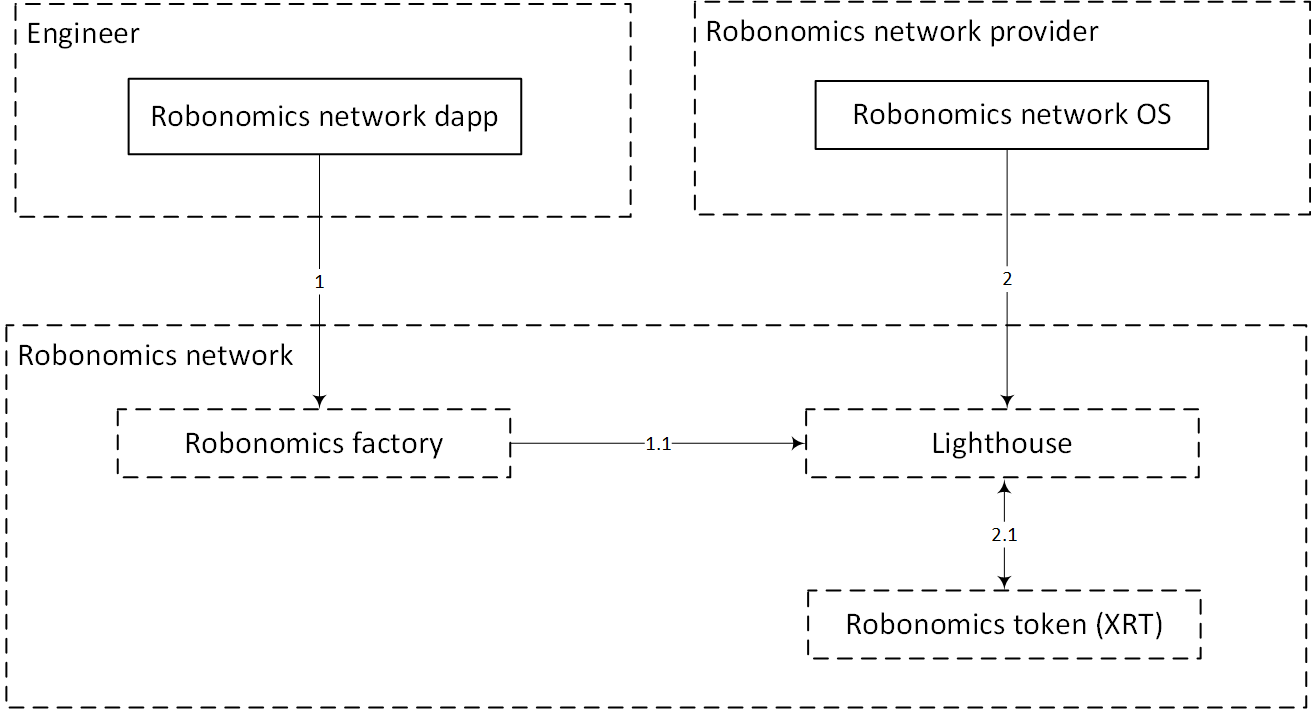
\includegraphics[width=1\textwidth]{step-by-step-2.png}

Robonomics网络提供商将事务(2)发送到创建的(1)灯塔,传输许多XRT代币(2.1)作为在提供者之间分配灯塔工作时间的容差。

\subsection{开始使用作为服务的网络物理系统}

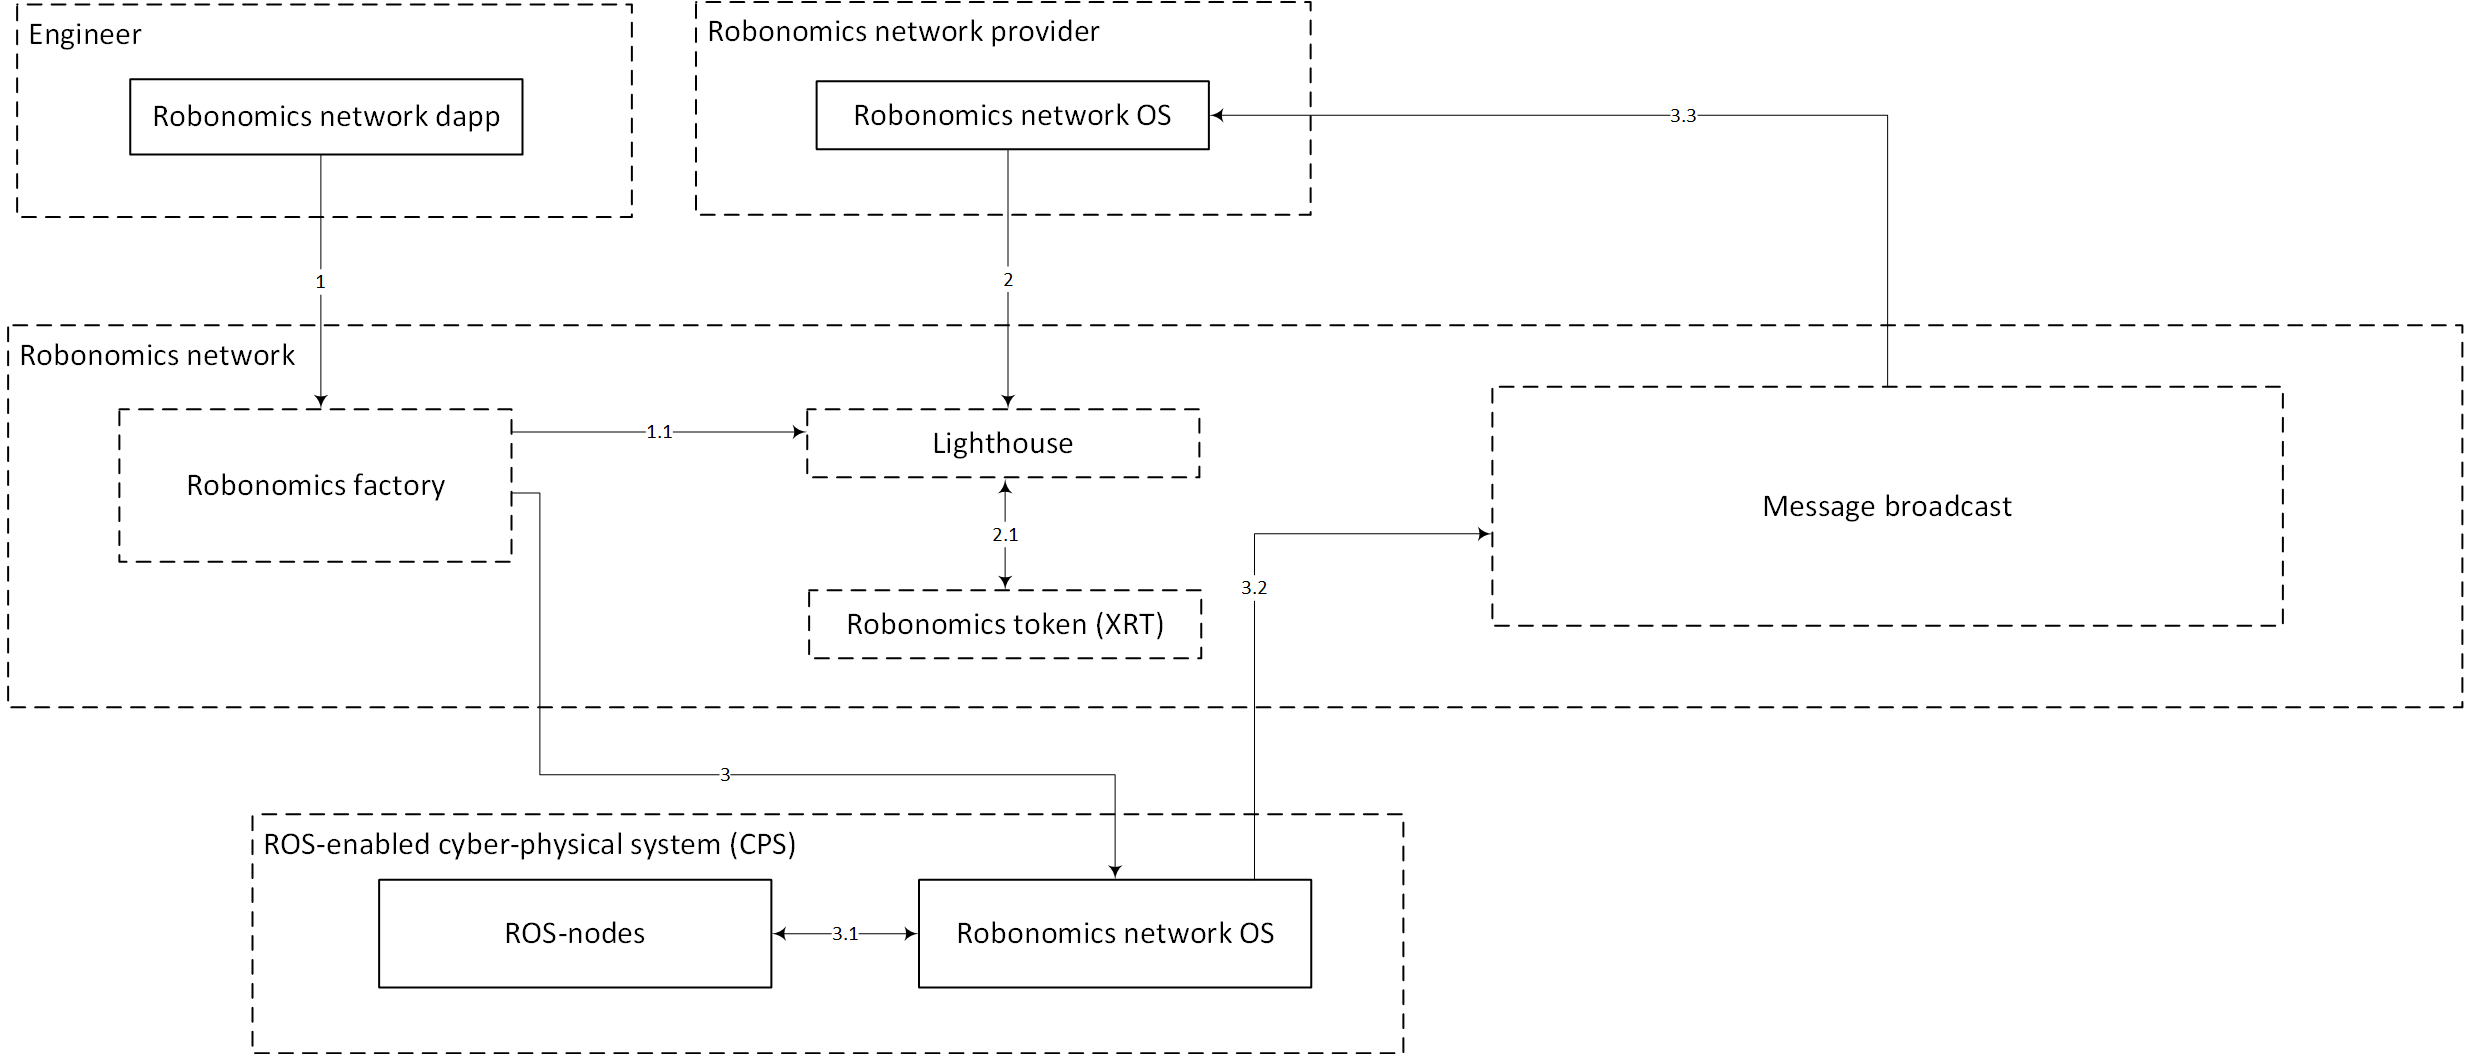
\includegraphics[width=1\textwidth]{step-by-step-3.png}

Robonomics网络操作系统收到Robonomics工厂创建的灯塔列表(3)。 使用来自灯塔描述和寻址其节点(3.1)的信息,CPS开始公布其为Robonomics广播频道提供服务的提议。

Robonomics网络提供商通过广播频道接收CPS发布新报价的消息(3.3)。

\subsection{Robonomics网络中用户的外观}

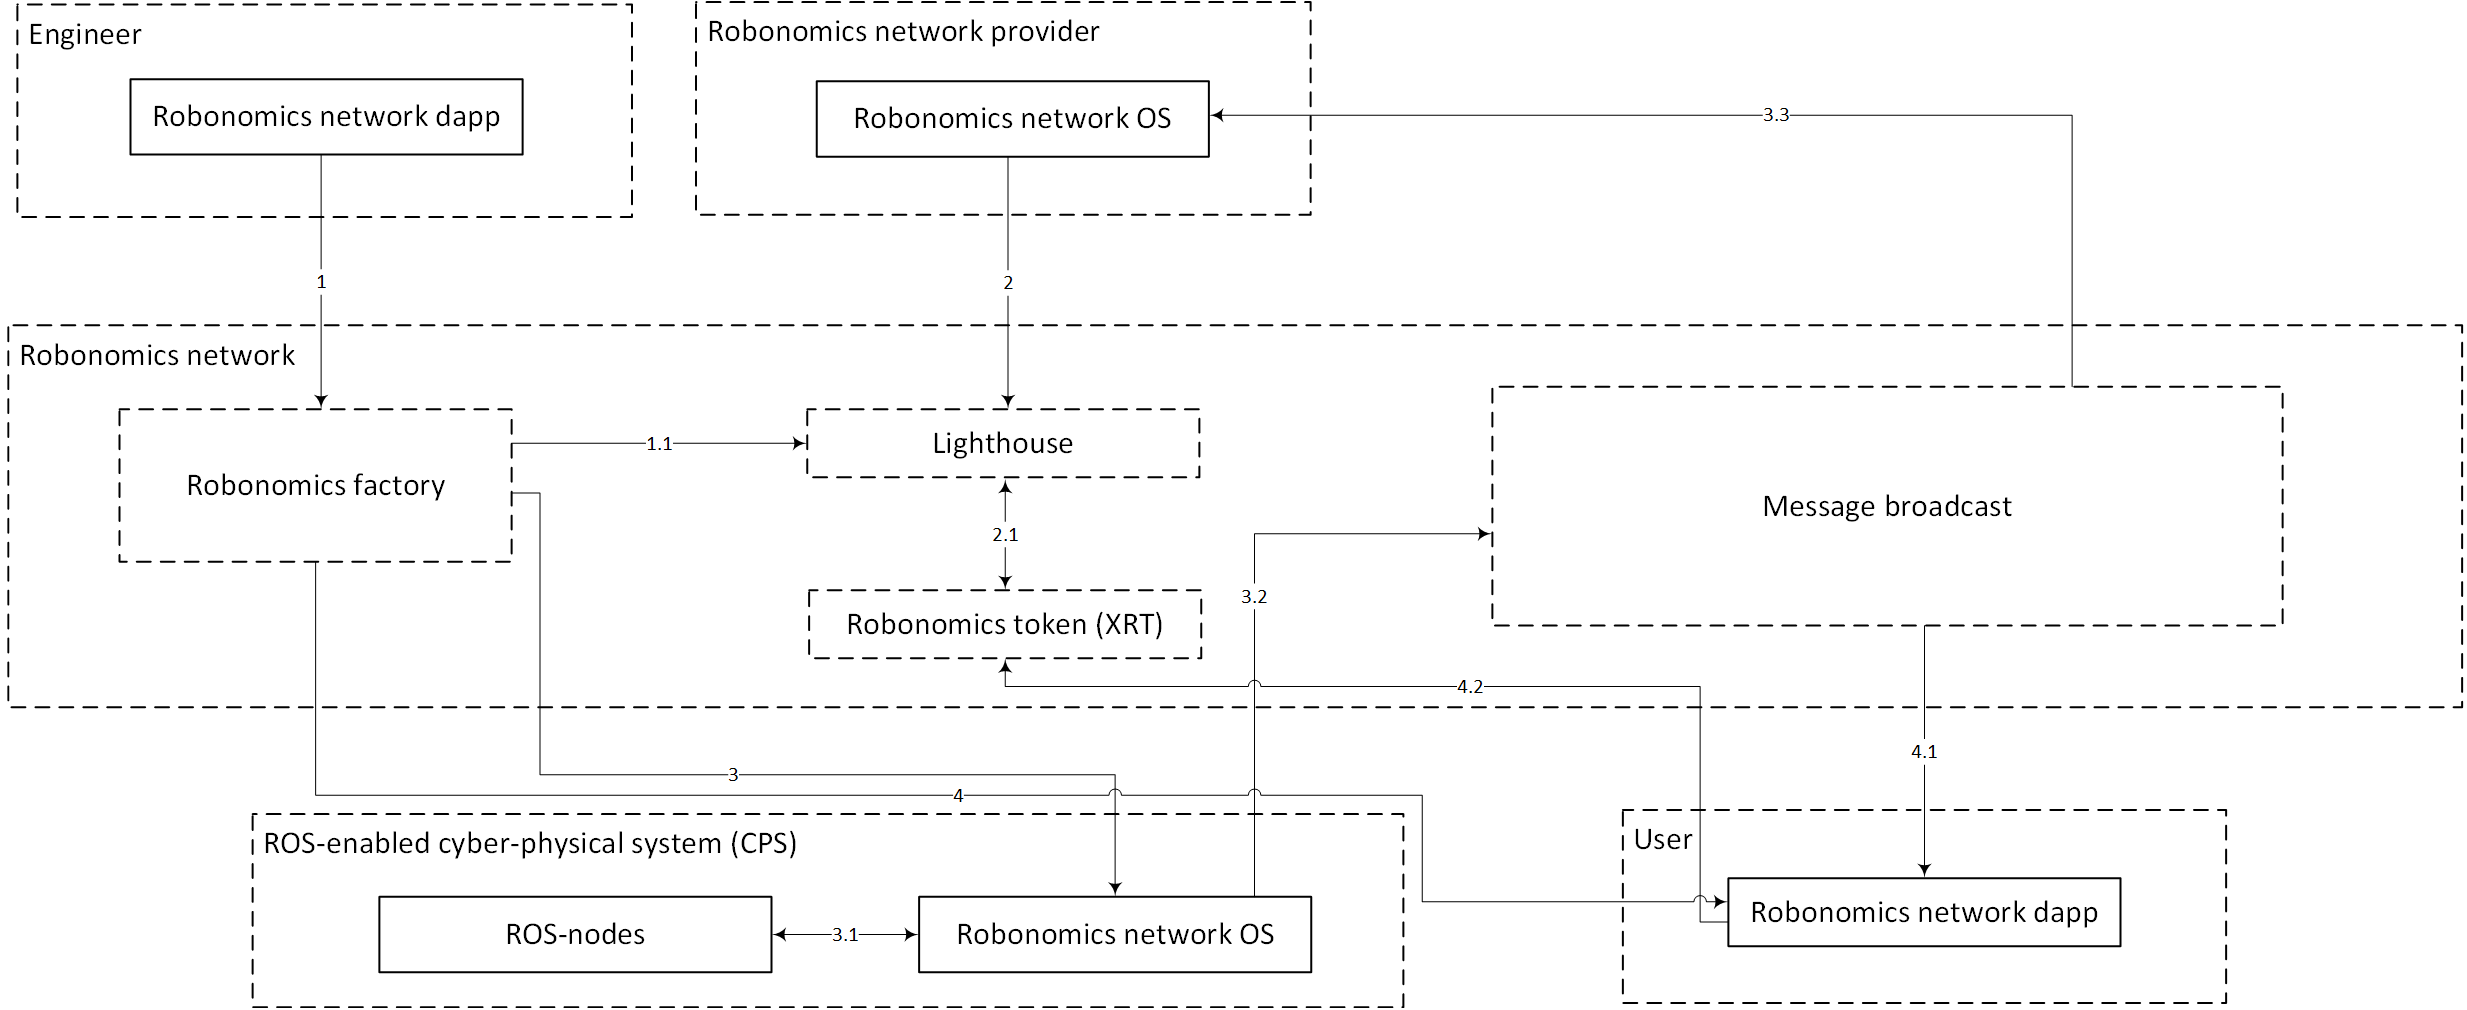
\includegraphics[width=1\textwidth]{step-by-step-4.png} 

用户在dapp的帮助下接收Robonomics广播频道列表(4)并开始收听这些频道中的消息(4.1)。 用户确保他对Robonomics网络感兴趣的CPS(3.2)提供服务,向以太坊区块链发送交易,以便通过Robonomics工厂的自主工作流程撤销XRT令牌(4.2)。

\subsection{创建由网络物理系统执行服务的责任}

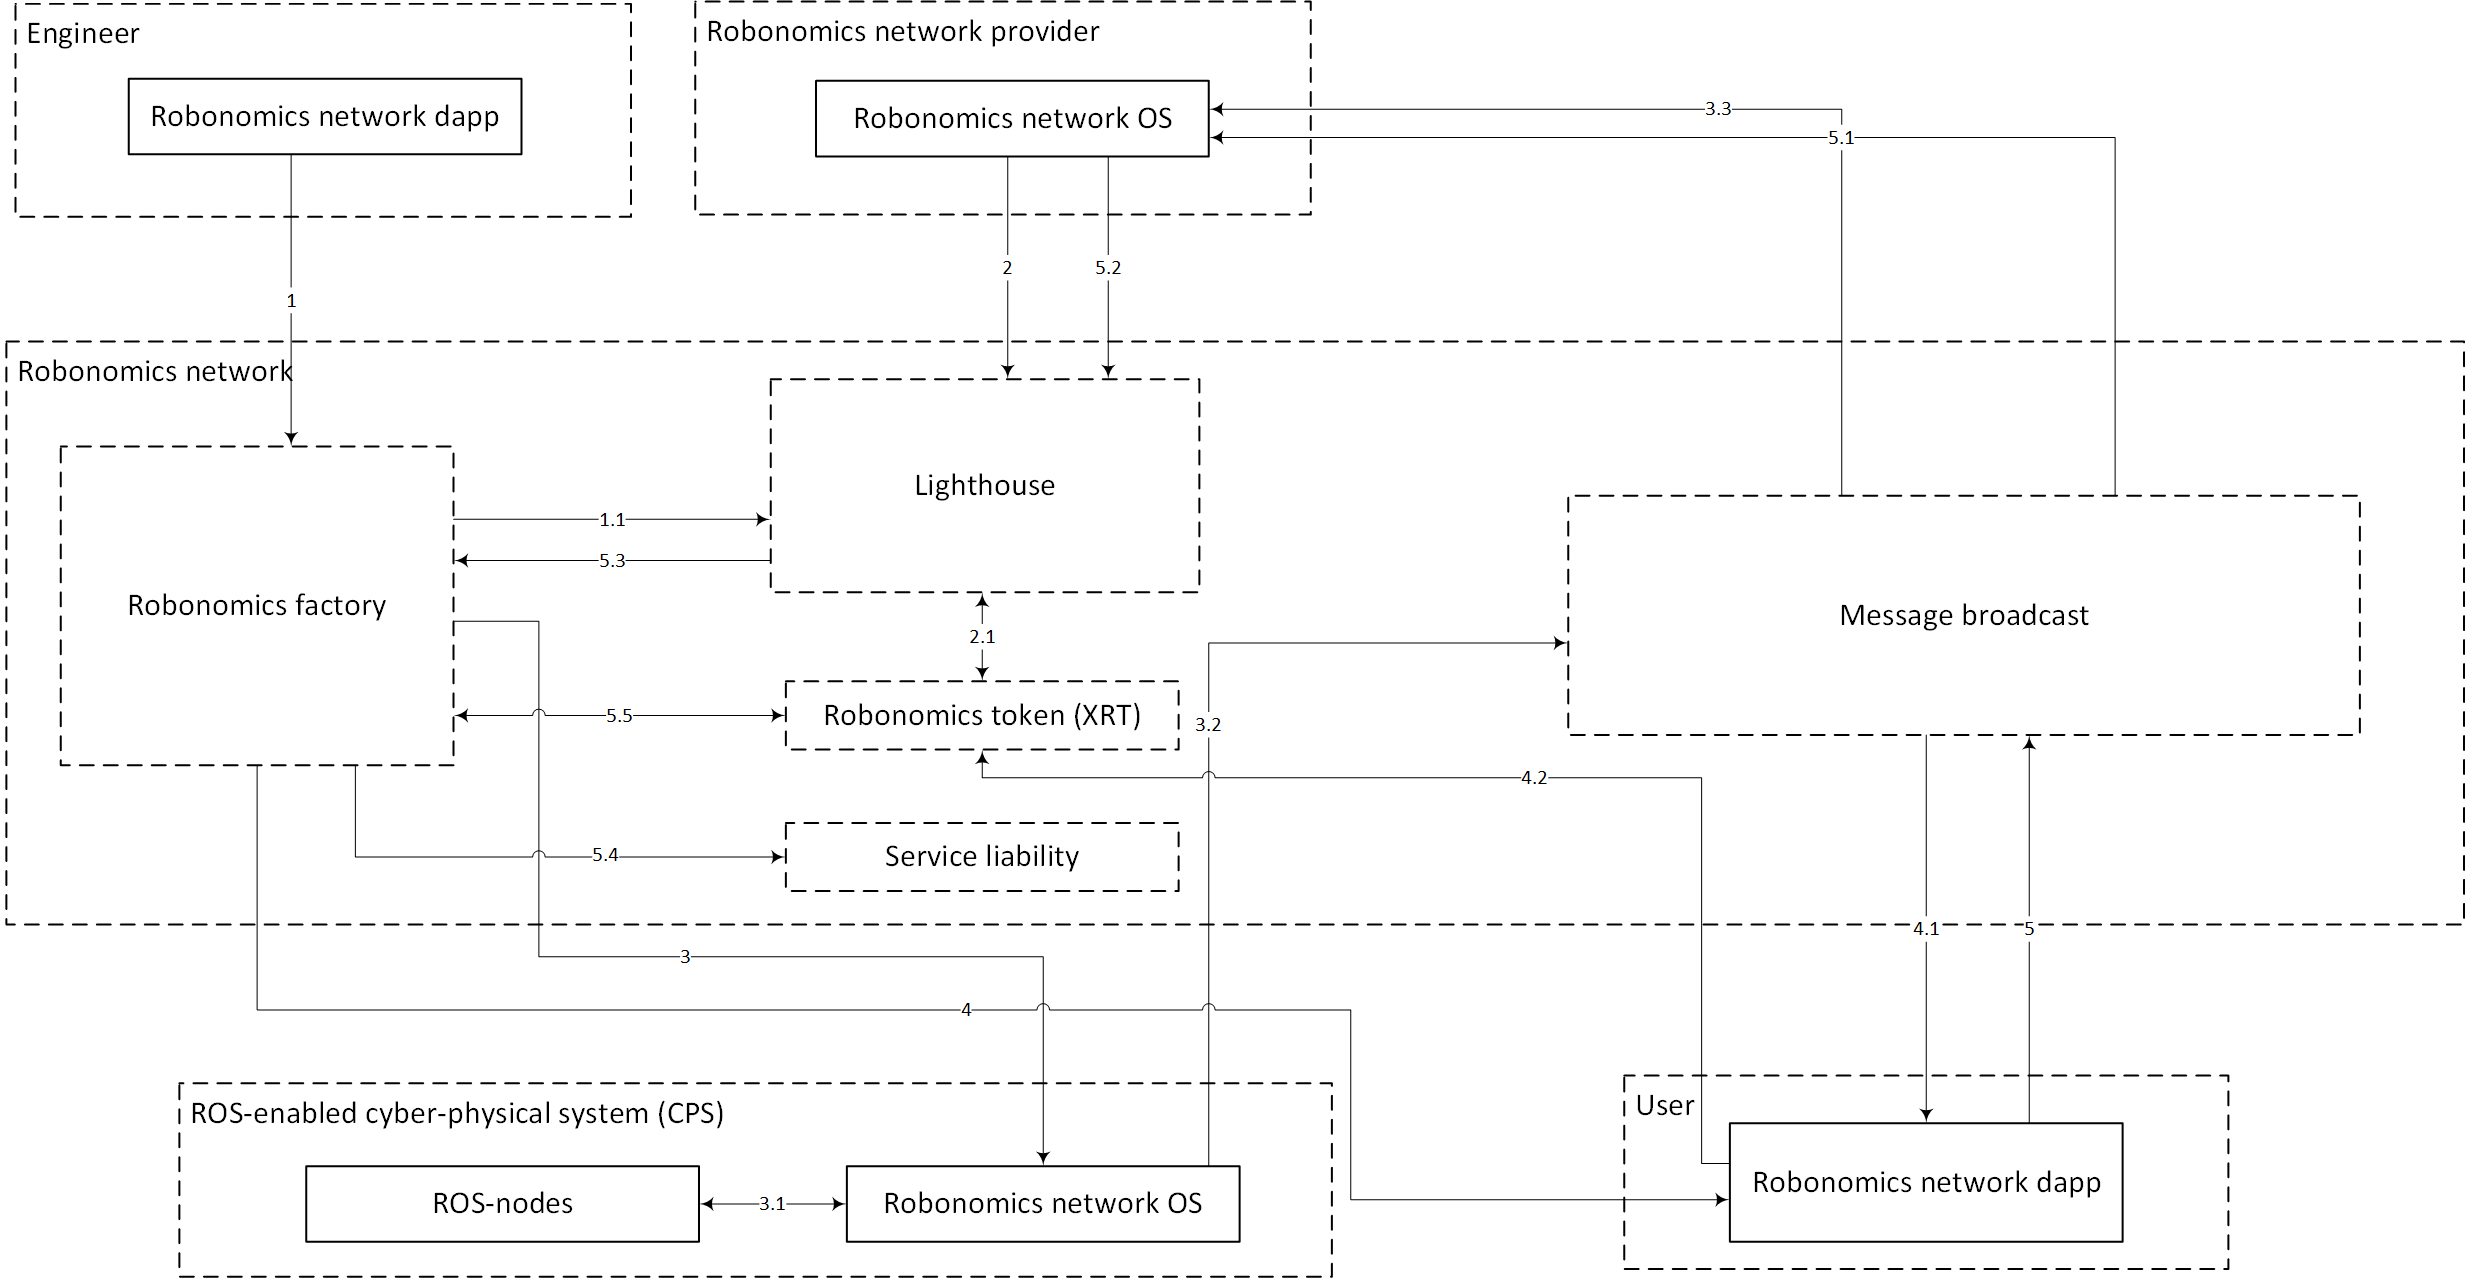
\includegraphics[width=1\textwidth]{step-by-step-5.png} 

具有足够的XRT令牌以对他感兴趣的服务提出要求的用户可以向广播中的先前发布的CPS服务(4.2)发送关于他的需求(5)的消息。

Robonomics网络提供商已收到用户的消息(5.1)并维护来自CPS(3.3)的本地存储消息,该消息与来自ROS兼容CPS的行为模型的哈希值和所提供服务的成本相匹配,参考 到灯塔的自主工作流程(5.2)传递双方的延期签名。

该灯塔致使Robonomics工厂(5.3)通过创建责任合同并知道其在以太坊区块链上的地址来创建服务(5.4),工厂的责任,解决XRT合同(5.5):
\begin{enumerate}
	\item 将服务成本从用户帐户(4.2)转移到合同帐户;
	\item XRT代币到合同账户的排放,即所需的总金额利用以太坊区块链上的起始因子乘以气体。
\end{enumerate}

\subsection{由网络物理系统执行的责任}

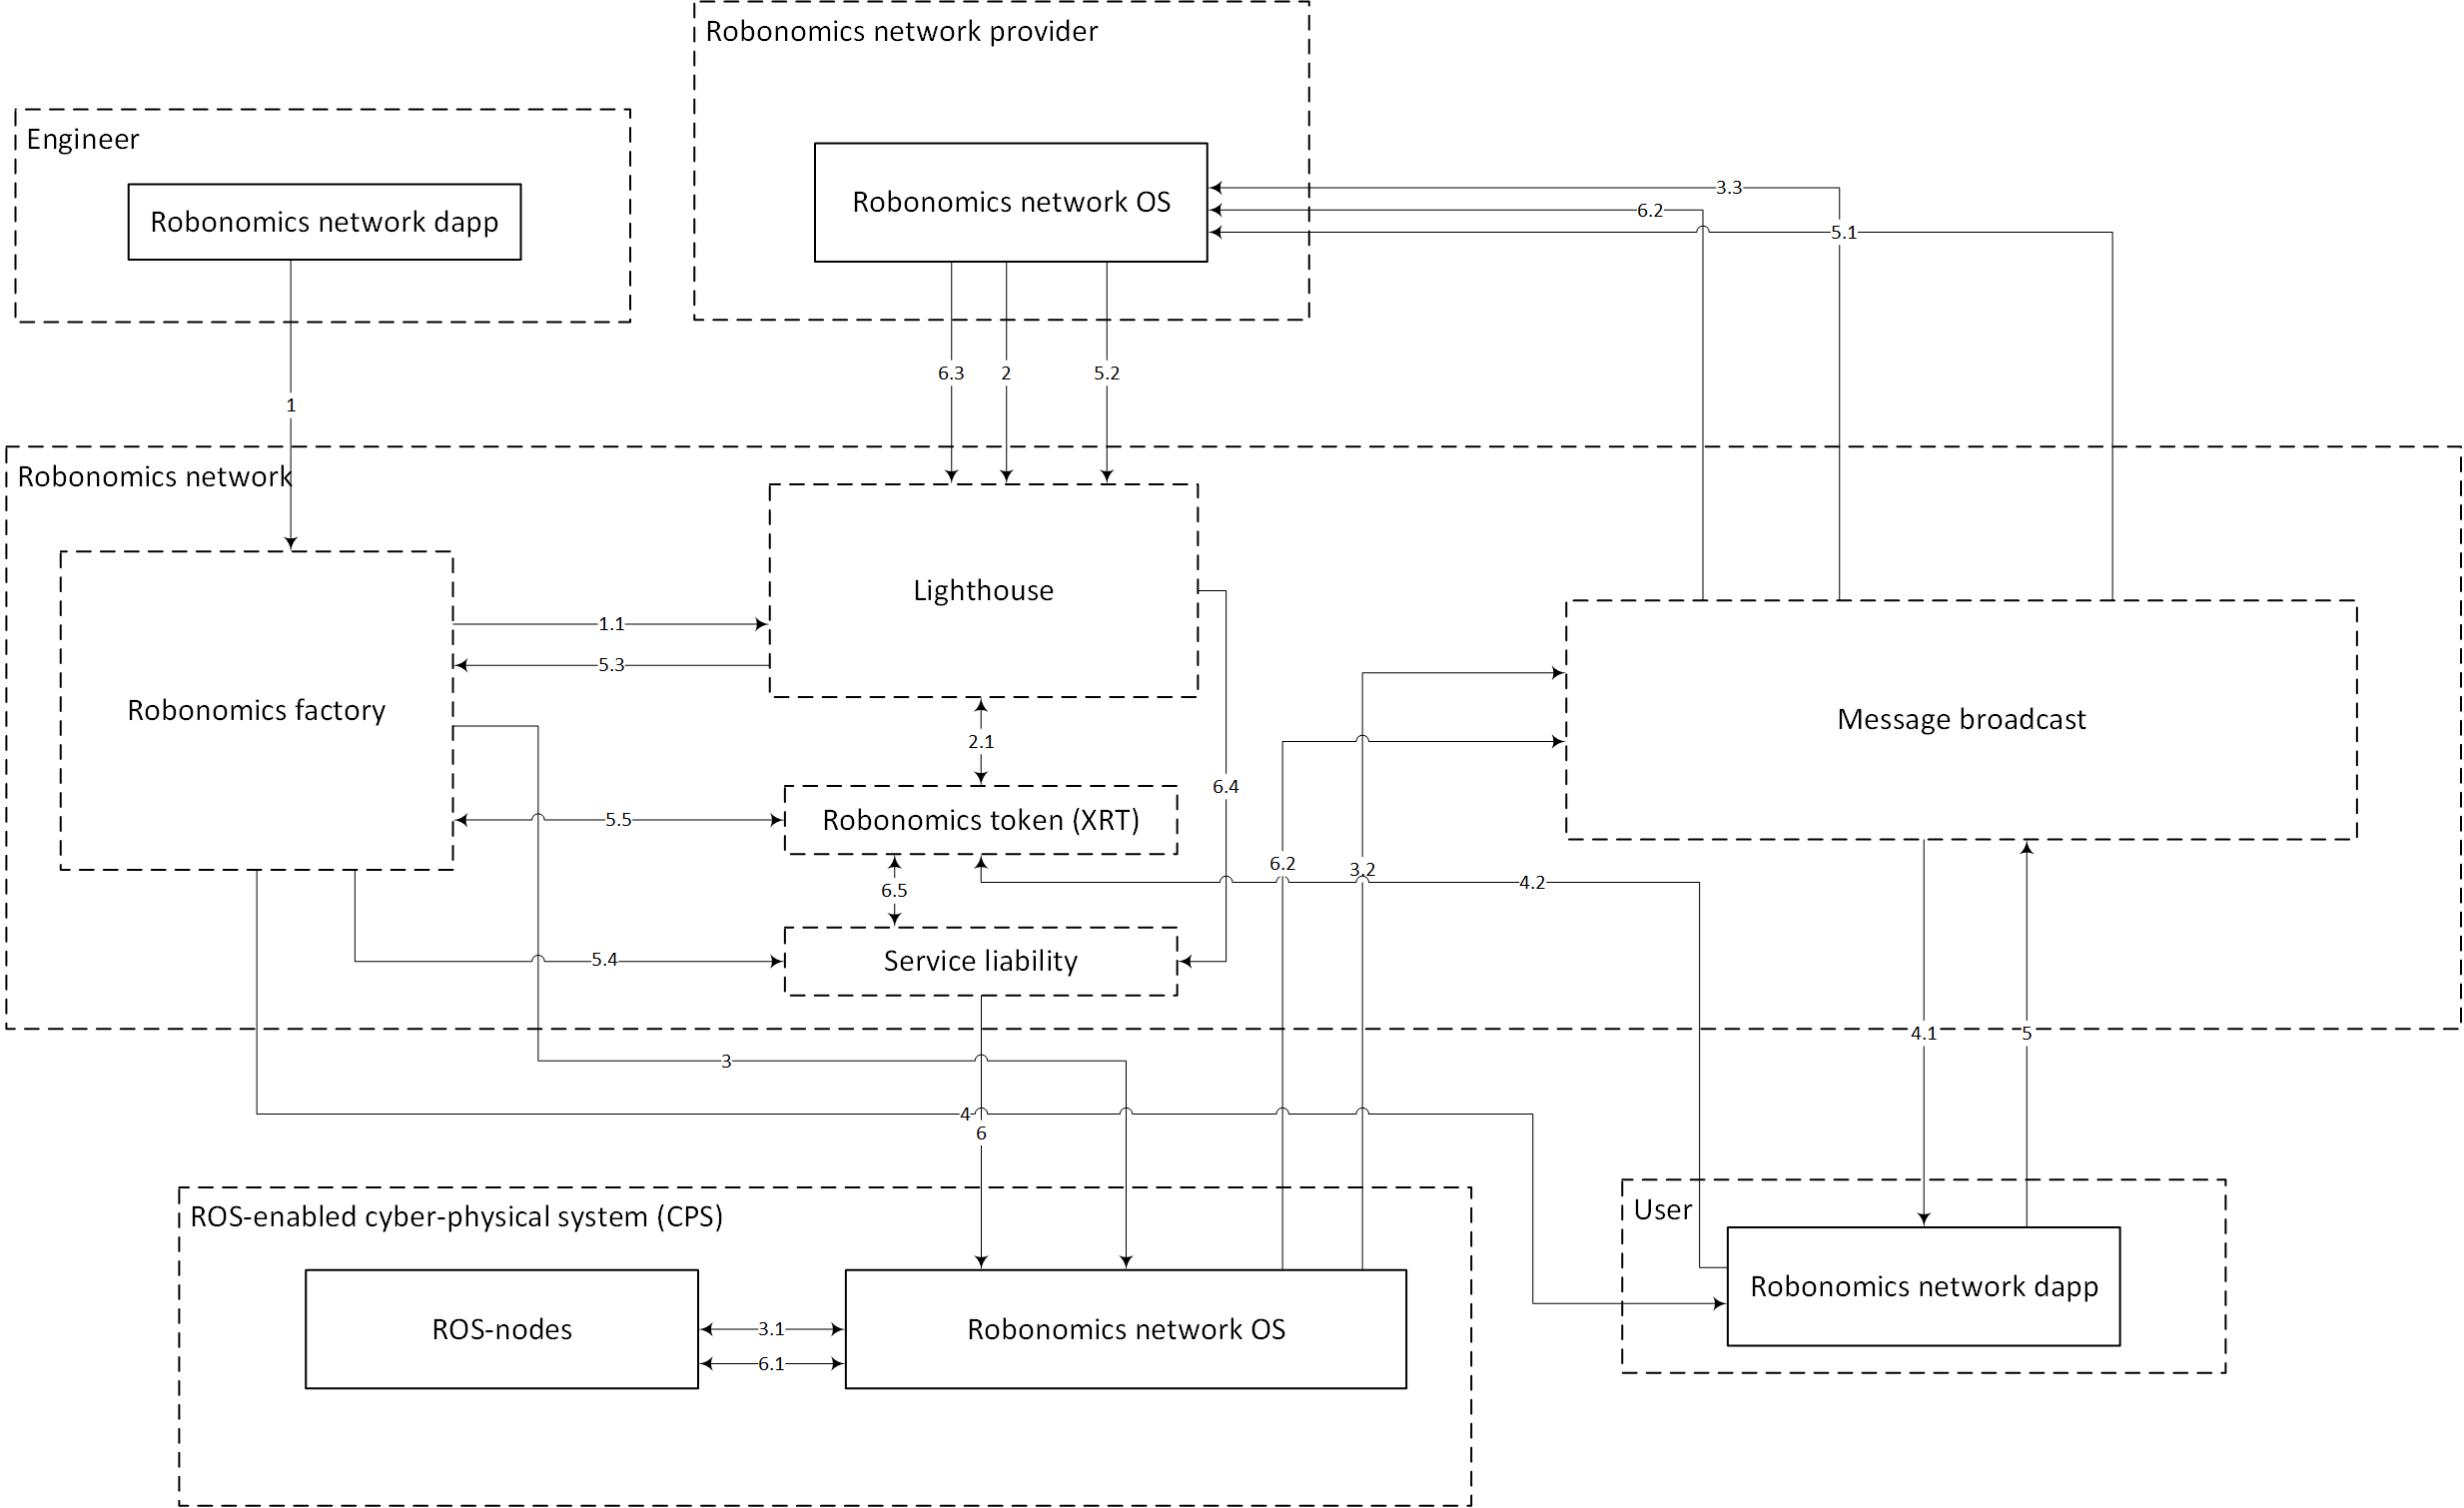
\includegraphics[width=1\textwidth]{step-by-step-6.png} 

网络物理系统在Robonomics网络操作系统的帮助下接收有关为其创建的责任合同的通知,其中可以找出行为模型的散列和行为模型的参数(变量)的散列(6)。

上传了行为模型和参数(6.1)以供执行后,CPS在ROS-bag的帮助下开始执行收到的责任。

在执行期间,CPS形成操作日志,并且在完成工作之后将其散列发送到服务于该行为模型的Robonomics通信信道(6.2)。

Robonomics网络提供商接收日志的散列(6.2),并通过以太坊区块链中的CPS(6.3)向灯塔(Lighthouse)发送关于履行责任的交易(6.3)。 灯塔为相应的服务责任创建内部交易,并在那里找到CPS操作日志(6.4)的散列。 然后,责任合同将提供的服务的费用下放到CPS地址,并将XRT发送到将交易发送到灯塔的提供商的地址。

\section{Robonomics平台应用程序}

\subsection{建立对智能城市和智能工厂生产的信任}

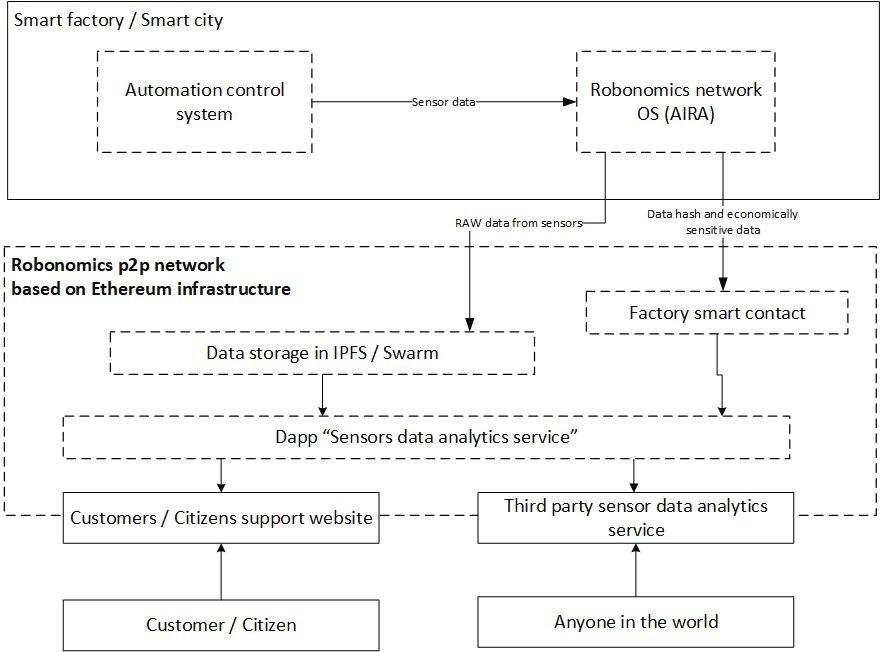
\includegraphics[width=1\textwidth]{app-1.png} 

消费者和智能工厂之间的信任问题在于消费者如何确定智能工厂生产的产品的质量。 商店里的产品可能很相似,但却有着截然不同的故事。 我们建议记录技术过程,将其置于分散的网络中。 来自CPS操作日志的哈希保存在区块链中,使产品的历史具有免疫性。 消费者对该产品充满信心,因为其历史未来不会改变。

\url{https://github.com/airalab/robonomics_comm/blob/master/robonomics_liability/src/robonomics_liability/executor.py#L50}

在这里,生产过程的数据是在智能工厂履行责任时收集和累积的。


\begin{lstlisting}
 {
	msg.result = self.ipfs.add(result_file)['Hash']
	self.complete.publish(msg)
  }
\end{lstlisting}


操作日志存储在IPFS网络中,其哈希值在合同责任中发布,将来不能更改。

\subsection{智能工厂由用户推出}

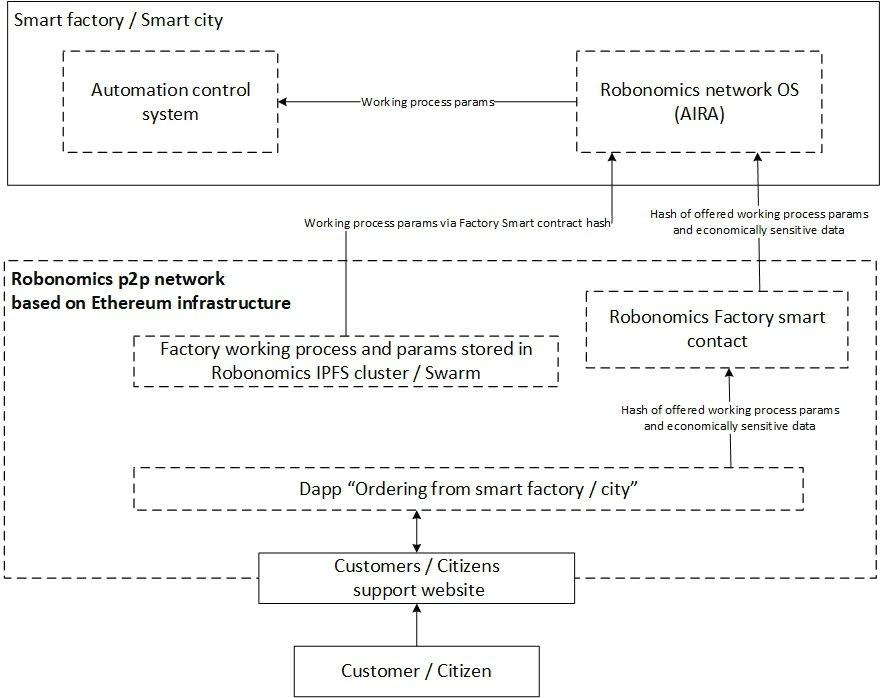
\includegraphics[width=1\textwidth]{app-2.png} 

作为消费者的服务访问工厂的问题在于消除可能以某种方式影响他们的交互的中介。 在这方面,智能合约是一个合适的对象。

\url{https://github.com/airalab/robonomics_comm/blob/master/robonomics_liability/src/robonomics_liability/executor.py#L34}

在这里,智能工厂跟踪智能合约工厂的事件,接受其被列为执行人的责任。

\begin{lstlisting}
rospy.logdebug('Getting objective %s...', msg.objective)
self.ipfs.get(msg.objective)

player = Player(msg.objective)
player.start()
\end{lstlisting}

一旦承担责任,智能工厂通过从IPFS下载责任参数并在本地再现其序列来开始执行。

\subsection{借助资本管理机器人的经济}

让我们设想一组经济上独立的网络物理系统或仅仅将机器人作为向量(R),将资本(投资)作为向量(K)。 这里矢量$ R = {R_i, i=\overline{1,n}}$其中市场上的$R_i$机器人数量,n检查市场的数量。 并且向量$ K = {K_j, j=\overline{1,n}} $,$K_j$投资到第j个市场。 让我们描述市场中机器人分布与资本成比例的模型如下:

\[
R'[k] = K[k] * { \sum R_i[k] \over \sum K_i[k] }
\]
\[
e[k] = R'[k] - R[k-1] ;
\]
这里:
\begin{itemize}
\item $R'[k]$ 市场中机器人所需的分布[编号];
\item $R[k-1]$ 该资本市场已经存在的机器人数量;
\item e 分布误差向量(偏离所需的分布值)[数量];
\item $i \in \overline{1,n}$  市场指数;
\item k 离散时间步长;
\item $\sum R_i[k] $ - 步骤k中所讨论的所有市场中的机器人数量;
\item $\sum K_i[k] $ - 步骤k中有关市场的投资额。
\end{itemize}

基于上述描述,我们可以制定如下管理机器人经济的规律:

每个机器人都应该努力参与分销错误较高的市场 \cite{LonshakovSergey2017HowProtocol}。

当下一个机器人被纳入经济体时,该机器人提供其报价的市场可从以下等式中选择:

$ i = maxi(e[k])$, 这导致 $ e_i[k] \rightarrow 0 $.

这里 $ maxi(e) $ - 偏差矢量的最大元素的索引。

\subsubsection{参考实施}

Robonomics管理算法的实现包含在机器人经济包控件中

\url{https://github.com/airalab/robonomics_comm/tree/master/robonomics_control}. 

在这里,线性分布算法基于来自智能合约的关于资本分配的信息和来自市场的关于从网络物理系统接收的批次的信息。

\url{https://github.com/airalab/robonomics_comm/blob/master/robonomics_control/src/robonomics_control/distribution.py}

\subsection{基于机器人劳动的代币化价值}

考虑智能城市中传感器释放碳单位的情景。 如果空气污染低于某个值,传感器有权发出碳单位的标记。 让传感器由于责任测量空气污染程度发送的碳单位数量,以及结果。 我们通过一种方法来扩展标准责任合同,该方法将排放单位数量与工作结果一起计算。
\begin{lstlisting}
function setResult(bytes32 _result, uint256 _emission);
\end{lstlisting}

这样,碳单位释放的价值保留在责任合同中。 如果观察员网络确认传感器测量结果是正确的,则根据责任合同将发出相应数量的代币。

\begin{lstlisting}
function confirm() {
  ... 
  carbonToken.emission(emission);
}
\end{lstlisting}

重要的是将责任合同添加到可以访问令牌排放的组中,工厂在初始阶段进行排放。 然后,责任合同工厂必须拥有关于设定行为模型符合这种标记的信息,这些信息可以在成功履行责任时发出。

\section{可扩展性}

Robonomics旨在代表如此庞大的网络物理系统,例如整个工厂或城市。 以太坊网络的当前容量足以每天执行超过1,000个合同义务。 这足以满足:汽车购买者在宝马,保时捷和Avtovaz等几个汽车集团的网站上每日直接订购的组织。 为当前全球工业区的无人物流登记定期航线。 每日出版有关人口超过1,000,000人的世界所有城市的感官网络的环境状况报告。

\section{以太坊的Robonomics部分}

随着在以太坊网络中创建自己的细分市场的能力的引入,Robonomics可以形成一个具有更大容量的细分市场,并且还允许机器人可能的合同性能数量的多次增加。 这可以满足整个工业4.0的要求,交易成本超过1,000美元。

\section{结论}

Robonomics平台旨在解决大规模生产,城市生活和物流的全面机器人化的社会和经济任务。 该平台的主要应用涉及与智能城市和工厂的服务和产品建立信任相关的任务,提供直接用户访问自治网络物理系统和借助资金管理多代理系统。

Robonomics平台将扩展以太坊网络基础设施的功能,用于工业4.0,物联网和智能城市等领域。
\newpage
\printbibliography
\newpage
\section*{附录1:机器人与经济理论交界处的问题}

全自动化。 机器人进入每个人的生活是不可避免的。 机器能够执行人类无法访问的任务,它们在许多类型的操作活动中更有效,并且在今天的日常工作中节省了人们的时间。

机器人技术的发展已经到了一个阶段,在这个阶段,物理或逻辑上分离的机器人之间的通信问题有权决定哪些行动适合作为其存在的一部分。 机器世界中使用的技术扩展了机器人可用的解决方案范围,每次都可以提高其自治水平。
自动机器人的通信任务最明显地体现在工业4.0和物联网等理念中。 根据这项工作的作者,以下是自动机器人参与人类生活的最重要问题清单:

\begin{itemize}
	\item 如何建立对机器人服务生产的信任?
	\item 如果生产和物流过程不涉及人类,如何确保所有权转移给消费者?
	\item 窗外的全自动化企业如何理解人类不断变化的需求?
	\item 如何确保两个不同公司的机器人之间的直接互动?
	\item 如何对机器人的活动征税以及应该将其视为单独的机器人单位?
\end{itemize}

这些问题的答案的不同变体带来了不稳定性增加和世界体系可能崩溃的各种风险 - 这对于建立一个没有奴隶人工劳动地的社会来说是一项挑战。

\section*{附录2:AIRA分发}

Robonomics OS的锚(参考)实现是AIRA项目(https://github.com/airalab/aira)。AIRA分发基于NixOS GNU / Linux发行版,由开放社区开发,其中Airalab开发人员是其中的一部分。

\paragraph{NixOS}

来自包数据库nixpkgs的分支是分发的基础(\url{https://github.com/airalab/airalab-channels}),其中Airalab团队添加了重要的以太坊基础设施包(如parity,web3.py); 支持机器人操作系统,以及Robonomics通信栈的基本包:robonomics市场,robonomics责任。

\paragraph*{ROS}

最小ROS支持在ros\_comm元数据包中提供,使用必要的基本软件堆栈,用于ROS网络参与者之间的序列化和消息传递,调用服务并集成到单个Rosgraph名称空间中。

根据分布情况,形成了实验工厂的安装图像(\url{https://aira.life/cases/}):火车游戏,工业4.0正在使用中。

\section*{附录3:外部API AIRA}

\begin{tabular}{ l |l}
	/market/incoming/ask & 来自通信渠道的需求传入消息。 \\
	/market/incoming/bid & 来自通信渠道的供给传入消息。 \\
	/market/sending/ask & 来自通信渠道的需求外来消息。 \\
	/market/sending/bid & 来自通信渠道的供给外来消息。 \\
	/market/signing/ask & 需要签署的需求外来消息。 \\
	/market/signing/bid & 需要签署的供给外来消息。 \\
\end{tabular}

\section*{附录4:DAO计划}

\paragraph{代表机器人的经济作为分散的以太坊计算机的程序。}

为了获得分散的服务,您需要一台分散的计算机和一个适合其特定角色的程序。 能够为智慧城市和工业4.0使用以太坊网络基础设施的工作流程可以作为以太坊计算机的程序呈现。

让我们假设我们有一个名为“机器人经济网络”的程序,我们将其加载到以太坊区块链中进行存储。 该计划允许以太坊基础设施的成员在其虚拟机上运行“机器人经济网络”,从而在分散的环境中组织新服务,充当其提供者。

\paragraph{机器人之经济作为DAO}

自主工作流程及其承包商组成DAO。承包商不能影响DAO的工作,他只能按照说明操作。 经济激励措施应该支持表演者对全面实施工作流程的兴趣。 在以太坊区块链中没有后果的情况下,工作流程无法改变。

%\end{CJK}
\end{document}
